\documentclass[10pt]{article}

\def\Type{LessonCaelan}
\def\TypeNum{Lesson 21}
\def\TypeTitle{Continuous Random Variables\\Solutions}
\def\Semester{Fall 2021} %Not Used 
\def\Course{MATH 1190 \& 1210}

\usepackage{preambleDJ}



%%%%%%%%%%%% BEGIN DOCUMENT %%%%%%%%%%%%%%%
%%%%%%%%%%%% BEGIN DOCUMENT %%%%%%%%%%%%%%%
%%%%%%%%%%%% BEGIN DOCUMENT %%%%%%%%%%%%%%%
%%%%%%%%%%%% BEGIN DOCUMENT %%%%%%%%%%%%%%%
%%%%%%%%%%%% BEGIN DOCUMENT %%%%%%%%%%%%%%%

\begin{document}


\thispagestyle{firstpage}
\pagestyle{otherpages}
\vs{0.5}

%\Heading{MATH 1190 \& 1210 Survey of Calculus I}{\begin{minipage}{0.25\textwidth}\begin{center} Lesson 20\\ Introduction to Probability \end{center}\end{minipage}}

\textbf{Intended Learning Outcomes}
After this lesson, you will be able to 

\begin{itemize}
\item Determine if a random variable is discrete or continuous. (\target{P1}, \target{P2})
\item Define support for a continuous random variable. (\target{P2})
\item List and apply properties of the probability density function of a continuous random variable. (\target{P2})
\item Find the formula and the graph of the cumulative distribution function of a continuous random variable. (\target{P2)}
\end{itemize}

\vspace{-0.5cm}

\hrulefill

\minil
We have seen {\em discrete random variables} have outcomes that are {\em countable}  (e.g. $1$,$2$,$3$, $\dots$.) Frequently there will only be a {\em finite} number of these values.\\
\blue{\bf Example} Last time we saw an example where $X$ was the (random) sum after rolling $2$ six-sided dice. We saw
\itemI{
\item Possible outcomes are $\ds \{ 2,3,4,5,6,7,8,9,10,11,12\}$ (tick marks on $x$-axis below)
\item The {\em probability mass function, $p(x)$} describes the probability for each outcome.  %%Need to add better description. Maybe a step function???
\item The probability of each outcome can also be represented by the areas of each bar in the histogram below, assuming the width of each bar is $1$.
} 
What happens if examine the sum of  many, many, many dice?
~\\
\hs{-.3}\mpageTth{.35}{.35}{.35}[\hs{.15}][\hs{.15}]{
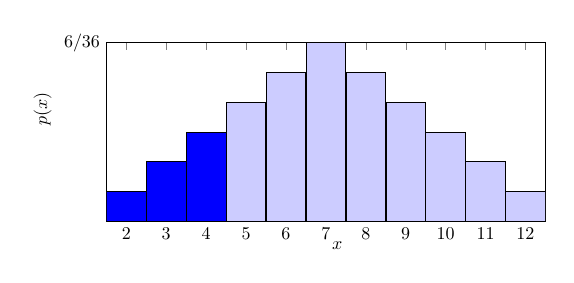
\begin{tikzpicture}[scale=0.65]
\begin{axis}[
%ymin=0, % Ensures bars start from zero
	xtick={1,	2,	3,	4,	5,	6,	7,	8,	9,	10,	11}, % Places x-axis ticks at data points
	xticklabels={
         2,	3,	4,	5,	6,	7,	8,	9,	10,	11,	12
         }, % Custom x-axis labels
	ytick       = {6/36},
	yticklabels =  {$6/36$},
enlarge x limits={.05}, % Adjusts spacing between bars and axis limits
	y label style={anchor=south west},
	ylabel={$p(x)$},
	xlabel = {$x$},
	x label style={anchor=west},
	%xticklabel style = {font=\small}, 
	ymin = 0, ymax = .167,
	width = 4in, height=2in,
	axis line style={->},
]
% \addplot[fill=blue!20] coordinates {(1,0)  (2,0)  (3,0) (4,0) (5,0) (6,0) (7,0) (8,0) (9,0) (10,0) (11,0)};
\addplot[ybar, bar shift=0,   bar width=22pt,  fill=blue!20] plot coordinates {
(1 , 0.02777778)	(2 , 0.05555556)	(3 , 0.08333333)	(4 , 0.11111111)	(5 , 0.13888889)	(6 , 0.16666667)	(7 , 0.13888889)	(8 , 0.11111111)	(9 , 0.08333333)	(10 , 0.05555556)	(11 , 0.02777778)
};
\addplot[ybar, bar shift=0,   bar width=22pt,  fill=blue] plot coordinates {
(1 , 0.02777778)	(2 , 0.05555556)	(3 , 0.08333333)	};
%	  \addplot[domain=0.5:1.5,  red, ultra thick, -, ] { 0.02777778 };
\end{axis}
\end{tikzpicture}
\centering
\parbox{1.2\textwidth}{\centering Histogram for Sum of $n=2$ dice}
}{
%
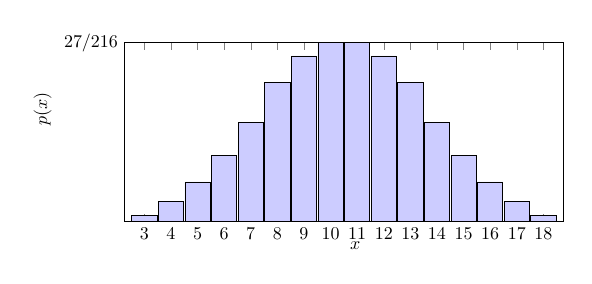
\begin{tikzpicture}[scale=0.65]
\begin{axis}[
%ymin=0, % Ensures bars start from zero
	xtick={1,	2,	3,	4,	5,	6,	7,	8,	9,	10,	11,	12,	13,	14,	15, 16}, % Places x-axis ticks at data points
	xticklabels={
         3,	4,	5,	6,	7,	8,	9,	10,	11,	12,	13,	14,	15,	16,	17, 18
         }, % Custom x-axis labels
	ytick       = {27/216},
	yticklabels =  {$27/216$},
	enlarge x limits={0.05}, % Adjusts spacing between bars and axis limits
	y label style={anchor=south west},
	ylabel={$p(x)$},
	xlabel = {$x$},
	x label style={anchor=west},
	%xticklabel style = {font=\small}, 
	ymin = 0, ymax = .125,
	width = 4in, height=2in,
	axis line style={->},
]
	% \addplot[fill=blue!20] coordinates {(1,0)  (2,0)  (3,0) (4,0) (5,0) (6,0) (7,0) (8,0) (9,0) (10,0) (11,0)};
	\addplot[ybar, bar shift=0,   bar width=14pt,  fill=blue!20] plot coordinates {
	(1 , 0.00462963)	(2 , 0.01388889)	(3 , 0.02777778)	(4 , 0.0462963)	(5 , 0.06944444)	(6 , 0.09722222)	(7 , 0.11574074)	(8 , 0.125)	(9 , 0.125)	(10 , 0.11574074)	(11 , 0.09722222)	(12 , 0.06944444)	(13 , 0.0462963)	(14 , 0.02777778)	(15 , 0.01388889) (16 , 0.00462963)
		};
\end{axis}
\end{tikzpicture}
\parbox{1.3\textwidth}{\centering Histogram for Sum of $n=3$ dice}
}{
%
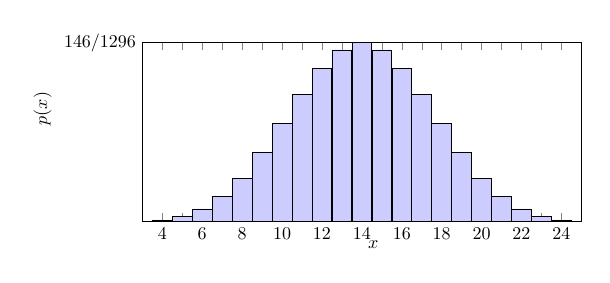
\begin{tikzpicture}[scale=0.65]
\begin{axis}[
	xtick={1,	2,	3,	4,	5,	6,	7,	8,	9,	10,	11,	12,	13,	14,	15,	16,	17,	18,	19,	20,	21}, % Places x-axis ticks at data points
	xticklabels={
         4,	,	6,	,	8,	,	10,	,	12,	,	14,	,	16,	,	18,	,	20,	,	22,	,	24
         }, % Custom x-axis labels
	ytick       = {146/1296},
	yticklabels =  {$146/1296$},
	y label style={anchor=south west},
ylabel={$p(x)$},
	xlabel = {$x$},
	enlarge x limits={0.05}, % Adjusts spacing between bars and axis limits
	x label style={anchor=west},
	%xticklabel style = {font=\small}, 
	ymin = 0, ymax = .113,
	width = 4in, height=2in,
	axis line style={->},
]
	% \addplot[fill=blue!20] coordinates {(1,0)  (2,0)  (3,0) (4,0) (5,0) (6,0) (7,0) (8,0) (9,0) (10,0) (11,0)};
	\addplot[ybar, bar shift=0, bar width=11pt,  fill=blue!20] plot coordinates {
	(1 , 0.0007716)	(2 , 0.00308642)	(3 , 0.00771605)	(4 , 0.0154321)	(5 , 0.02700617)	(6 , 0.04320988)	(7 , 0.0617284)	(8 , 0.08024691)	(9 , 0.09645062)	(10 , 0.10802469)	(11 , 0.11265432)	(12 , 0.10802469)	(13 , 0.09645062)	(14 , 0.08024691)	(15 , 0.0617284)	(16 , 0.04320988)	(17 , 0.02700617)	(18 , 0.0154321)	(19 , 0.00771605)	(20 , 0.00308642)	(21 , 0.0007716)
	};
\end{axis}
\end{tikzpicture}
\parbox{1.4\textwidth}{\centering Histogram for Sum of $n=4$ dice}    
}

\hs{-.3}\mpageTth{.35}{.4}{.35}[\hs{.15}][\hs{.15}]{
\parbox{1.5\textwidth}{\centering \hs{3.5}\,}   
\blue{
{\em Observations}\small
\itemI{
\item For the sum of $2$ dice,\al{
P(X\leq 4)=\sum_{k=2}^4 (P(X=k)\hs{.58}  \\
=P(X=2)+P(X=3)+P(X=4)
}
\item This equivalent to area of first $3$ bars histogram (see dark blue)
}
}
}{
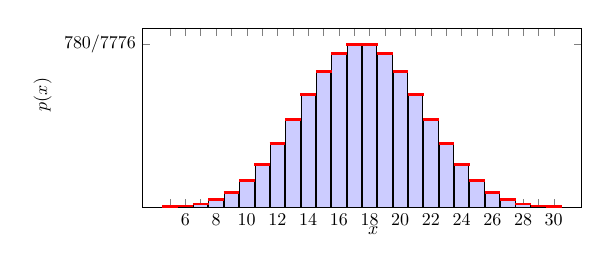
\begin{tikzpicture}[scale=0.65]
\begin{axis}[
%ymin=0, % Ensures bars start from zero
	xtick={1,	2,	3,	4,	5,	6,	7,	8,	9,	10,	11,	12,	13,	14,	15,	16,	17,	18,	19,	20,	21,	22,	23,	24,	25,	26}, % Places x-axis ticks at data points
	xticklabels={
         ,	6,	,	8,	,	10,	,	12,	,	14,	,	16,	,	18,	,	20,	,	22,	,	24,	,	26,	,	28,	,	30,
         }, % Custom x-axis labels
	ytick       = {780/7776},
	yticklabels =  {$780/7776$},
	enlarge x limits={.05}, % Adjusts spacing between bars and axis limits
	y label style={anchor=south west},
	ylabel={$p(x)$},
	xlabel = {$x$},
	x label style={anchor=west},
	%xticklabel style = {font=\small}, 
	ymin = 0, ymax = .1103,
	width = 4in, height=2in,
	axis line style={->},
]
	% \addplot[fill=blue!20] coordinates {(1,0)  (2,0)  (3,0) (4,0) (5,0) (6,0) (7,0) (8,0) (9,0) (10,0) (11,0)};
	\addplot[ybar, bar shift=0,   bar width=8pt,  fill=blue!20] plot coordinates {
(	(1 , 0.0001286)	(2 , 0.000643)	(3 , 0.00192901)	(4 , 0.00450103)	(5 , 0.00900206)	(6 , 0.0162037)	(7 , 0.02636317)	(8 , 0.03922325)	(9 , 0.05401235)	(10 , 0.06944444)	(11 , 0.08371914)	(12 , 0.0945216)	(13 , 0.10030864)	(14 , 0.10030864)	(15 , 0.0945216)	(16 , 0.08371914)	(17 , 0.06944444)	(18 , 0.05401235)	(19 , 0.03922325)	(20 , 0.02636317)	(21 , 0.0162037)	(22 , 0.00900206)	(23 , 0.00450103)	(24 , 0.00192901)	(25 , 0.000643)	(26 , 0.0001286)
	};
	 % \addplot[ domain=0:26,  red, ultra thick, <->, ] {1/sqrt(2*pi*(3.85)^2)*e^(-(x-13.5)^2/(2*(3.85)^2))  };
	 \addplot[domain=0.5:1.5, red, ultra thick] {0.0001286};
\addplot[domain=1.5:2.5, red, ultra thick] {0.000643};
\addplot[domain=2.5:3.5, red, ultra thick] {0.00192901};
\addplot[domain=3.5:4.5, red, ultra thick] {0.00450103};
\addplot[domain=4.5:5.5, red, ultra thick] {0.00900206};
\addplot[domain=5.5:6.5, red, ultra thick] {0.0162037};
\addplot[domain=6.5:7.5, red, ultra thick] {0.02636317};
\addplot[domain=7.5:8.5, red, ultra thick] {0.03922325};
\addplot[domain=8.5:9.5, red, ultra thick] {0.05401235};
\addplot[domain=9.5:10.5, red, ultra thick] {0.06944444};
\addplot[domain=10.5:11.5, red, ultra thick] {0.08371914};
\addplot[domain=11.5:12.5, red, ultra thick] {0.0945216};
\addplot[domain=12.5:13.5, red, ultra thick] {0.10030864};
\addplot[domain=13.5:14.5, red, ultra thick] {0.10030864};
\addplot[domain=14.5:15.5, red, ultra thick] {0.0945216};
\addplot[domain=15.5:16.5, red, ultra thick] {0.08371914};
\addplot[domain=16.5:17.5, red, ultra thick] {0.06944444};
\addplot[domain=17.5:18.5, red, ultra thick] {0.05401235};
\addplot[domain=18.5:19.5, red, ultra thick] {0.03922325};
\addplot[domain=19.5:20.5, red, ultra thick] {0.02636317};
\addplot[domain=20.5:21.5, red, ultra thick] {0.0162037};
\addplot[domain=21.5:22.5, red, ultra thick] {0.00900206};
\addplot[domain=22.5:23.5, red, ultra thick] {0.00450103};
\addplot[domain=23.5:24.5, red, ultra thick] {0.00192901};
\addplot[domain=24.5:25.5, red, ultra thick] {0.000643};
\addplot[domain=25.5:26.5, red, ultra thick] {0.0001286};
\end{axis}
\end{tikzpicture}
\parbox{1.2\textwidth}{\centering Histogram for Sum of $n=5$ dice}    
}{
\begin{tikzpicture}[scale=0.65]
\begin{axis}[
%ymin=0, % Ensures bars start from zero
	xtick={10,18}, %\empty, %{1,	2,	3,	4,	5,	6,	7,	8,	9,	10,	11,	12,	13,	14,	15,	16,	17,	18,	19,	20,	21,	22,	23,	24,	25,	26}, % Places x-axis ticks at data points
	xticklabels={10,18}, % Custom x-axis labels
	ytick       = \empty, %{780/7776},
	yticklabels =  {$780/7776$},
enlarge x limits={.05}, % Adjusts spacing between bars and axis limits
	y label style={anchor=south west},
	ylabel={$p(x)$},
	xlabel = {$x$},
	x label style={anchor=west},
	xticklabel style = {font=\small}, 
	ymin = 0, ymax = .1103,
	width = 4in, height=2in,
	axis line style={->},
]
	  \addplot[ name path=f, domain=0:26,  red, ultra thick, <->, ] {1/sqrt(2*pi*(3.85)^2)*e^(-(x-13.5)^2/(2*(3.85)^2))  };
	   \path[name path=axis] (0,0) -- (26,0);
	    \addplot [
                    thick,
                    color=blue!20,
                    fill=blue!20, 
                    ]
                    fill between[
                    of=f and axis,
                    soft clip={domain=0:26},
                    ];
                   	  \addplot[ name path=f, domain=10:18,  red, ultra thick, -, ] {1/sqrt(2*pi*(3.85)^2)*e^(-(x-13.5)^2/(2*(3.85)^2))  };
	   \path[name path=axis] (10,0) -- (28,0);
	    \addplot [
                    thick,
                    color=blue,
                    fill=blue, 
                    ]
                    fill between[
                    of=f and axis,
                    soft clip={domain=10:18},
                    ]; 
\end{axis}
\end{tikzpicture}
\parbox{1\textwidth}{\centering Histogram for Sum of $n\to\infty$ dice}   
}
\blue{
\itemI{
\item The graph of $p(x)$ is a discontinuous step function (see red in sum of $5$ dice).
\item As we consider the histogram of the sum of many, many, many dice (i.e. we let $n\to infty$) $p(x)$ becomes the continuous normal distribution (see graph in red on far right).
\item Big picture: For continuous random variables, we will still find probability by utilizing the area under the continuous $p(x)$ (see dark blue in histogram for $n\to \infty$ dice). For example $$P(10\leq X\leq 18)=\int_{10}^{18}p(x)\;dx$$
}
}
A {\em continuous probability distribution} is continuous because the set of outcomes of an experiment
is continuous. (e.g. measuring the height of a person, determining the wait time at the DMV,
weighing a Roots Bowl, etc).
\itemI{
\item Possible outcomes are an interval: $\ds (-\infty,\infty)$, $([0,1]$, $[0,100]$, etc.
\item The {\em probability density function} $p(x)$ is continuous and is used to find the probability for a range of outcomes.
\item The probability of between two values is equivalent to the area between $p(x)$ and the horizontal axis.
}


%\newpage

\textbf{\color{blue} Warm Up}\exercise{\bf\color{Orange}P1, P2} Determine whether each of the random variable in the following scenarios is discrete or continuous.

\begin{enumerate}[label=(\alph*)]
\item $X$ is the (random)  number of arrivals at an emergency room from midnight to 6am on a given day.
\sol{
$X$ is discrete since the number of arrivals  are $1,2,3,4$, et.c
}
\vfill
\item $T$ is the (random)  temperature of a cup of coffee from a coffee shop.
\sol{
$T$ is continuous since the temperature could be any value on an interval, say $0\leq T\leq 100$ $^\circ$C
}

\vfill 

\item $B$ is the number of boys in a randomly-selected family with 3 children.
\sol{
$B$ is discrete since $B$ will be $0$, $1$, $2$, or $3$.
}

\vfill
\end{enumerate}

%%%%%%%%%
\newpage%
%%%%%%%%%
\blue{\bf Key Properties of  Continuous Random Variables}\\
\mpageT{.5}{.5}[\hs{.1}]{
\centering
\blue{ \bf Discrete Random Variables}
}{
\centering
\blue{ \bf Continuous Random Variables}\\
}%\vs{-.2}
\itemNIN{
\mpageT{.5}{.5}[\hs{.2}]{
\item {\bf Discrete Example: } The random variable $X$ is the sum from randomly rolling two $4$-sided dice
}{
\item \blue{\bf Continuous}\example The random variable $T$ is the (random) wait time until the bus arrives  at the 
amphitheater on McIntyre. Buses arrive every $30$ minutes with evenly distributed probability (a uniform distribution)
}
\vs{.0}\\
\mpageT{.5}{.5}[\hs{.2}]{
\item The {\em Sample Space of $X$}: $S_X=\{2,3,4,5,6,7,8\}$
}{
\item The {\em Support of $T$}: $S_T=$ \blue{ $[a,b]=[0,30]$}
\\\\
$S=[a,b]$:  $[a,b]$ is smallest interval where $p(t)> 0$
}
\vs{.2}\\
\mpageT{.5}{.5}[\hs{.2}]{
\item {\bf Probability Mass Function}:  $p(x)$.\\
{ \em Two Properties:}
\enum{
\item $0\leq p(x)\leq 1$ where $x\in S_X$\vs{.3}
\item $\ds \sum_{k\in S_X}P[X=k] = \sum_{k=2}^8 P[X=k]=\sum_{k=2}^8 p(k)=1$
}
%
}{
\item {\bf Probability Density Function (PDF)}: $p(t)$.\\
{ \em Two Properties:}
\enum{
\item \blue{$p(t)\geq0$ where $t\in S_T$. Note that this differs from discrete random variables in that there is {\em not} a requirement that $p(t)\leq 1$.}
\item \blue{$\ds \int_a^b p(t)\;dt=\ds \int_0^{30} p(t)\;dt=1$ }
}
\vs{.1}
}

\mpageT{.5}{.5}[\hs{.2}]{
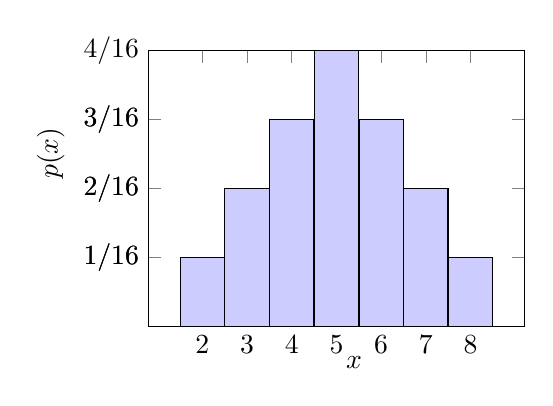
\begin{tikzpicture}
\begin{axis}[
%ymin=0, % Ensures bars start from zero
	xtick={1,	2,	3,	4,	5,	6,	7}, % Places x-axis ticks at data points
	xticklabels={
         2,	3,	4,	5,	6,	7,	8
         }, % Custom x-axis labels
ytick       = {1/16, 2/16, 3/16,4/16,3/16,2/16,1/16},
yticklabels =  {$1/16$, $2/16$, $3/16$,$4/16$,$3/16$,$2/16$,$1/16$},
enlarge x limits={.2}, % Adjusts spacing between bars and axis limits
	y label style={anchor=south west},
	ylabel={$p(x)$},
	xlabel = {$x$},
	x label style={anchor=west},
	%xticklabel style = {font=\small}, 
	ymin = 0, ymax = .25,
	width = 2.5in, height=2in,
	   axis line style={->},
]
% \addplot[fill=blue!20] coordinates {(1,0)  (2,0)  (3,0) (4,0) (5,0) (6,0) (7,0) (8,0) (9,0) (10,0) (11,0)};
\addplot[ybar, bar shift=0,   bar width=16pt,  fill=blue!20] plot coordinates {
(1,.0625)  (2,.125) (3,.1875) (4,.25) (5,.1875) (6,.125) (7,.0625) 
};
\end{axis}
\end{tikzpicture}
}{
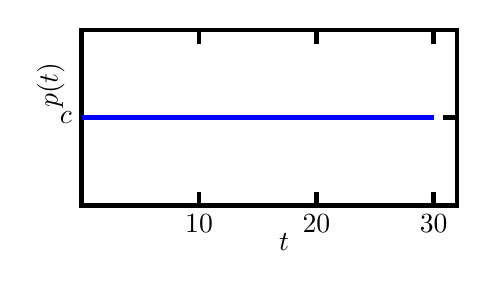
\begin{tikzpicture}
\begin{axis}[
	x label style={anchor=west},
xlabel={$t$},
xtick       = {10,20,30},
%xticklabels = {$10$,$20$,$30$},
xticklabel style={anchor=north},
y label style={anchor=west},
ylabel={$p(t)$},
%ytick=\empty,
%ytick       = {1/30},
ytick={0.05},
yticklabels = {$c$},
samples     = 320,
%domain      = -2.5:2.5,
%restrict y to domain=-6.5:6.5,
xmin =0, xmax = 32,
ymin = 0, ymax = .1,
axis line style = { ultra thick, -},
every major tick/.append style={ultra thick, black, major tick length=5pt},
width=2.5in, height=1.5in
%  grid=both, grid style=solid
]
  \addplot[domain=0:30, blue, ultra thick, mark=none]{.05};
%    \addplot[domain=0:5, blue, ultra thick, mark=none]{1/25*x};
%     \addplot[domain=5:10, blue, ultra thick, mark=none]{-1/25*x+2/5};
\end{axis}
\end{tikzpicture}
}
}
\tasksA{2}{
\task What is the support of $T$?
\sol{
$0\leq t\leq 30$
}




\task What is the value of $c$ in the above graph?. Hint: Consider how property $\#2$ for continuous random variables might be helpful.
\sol{
Property $\#2$ for continuous random variablesL $\ds \int_a^b p(t)\;dt=1$. Since $[a,b]=[0,30]$ and $p(t)=c$, we need
\al{
\int_0^{30} c\;dt&=1\\
c \cdot t\Bigg|_0^{30}&=1\\
c\cdot 30-c\cdot0&=1\\
30c&=1\\
c&=\frac{1}{30}
}
}
\task* Use $p(t)$ and an integral to find $P(T\leq 10)$, the probability that this person waits for no more than 10 minutes.\\
\mpageT{.5}{.5}{
\sol{
\al{
P(T\leq 10)&=\int_0^{10} \frac{1}{30}\;dt\\
&=\frac{1}{30}\cdot t\Bigg|_0^{10}\\
&=\frac{1}{30}\cdot 10-\frac{1}{30}\cdot 0\\
&=\frac{10}{30}\\
&=\frac{1}{3}
}
There is a $\ds \frac{1}{3}=33.3\bar{3}\%$ probability of waiting $10$ minutes or less.
}
}{
\begin{center}
\begin{tikzpicture}
\begin{axis}[
	x label style={anchor=west},
xlabel={$t$},
xtick       = {10,20,30},
%xticklabels = {$10$,$20$,$30$},
xticklabel style={anchor=north},
y label style={anchor=west},
ylabel={$p(t)$},
%ytick=\empty,
%ytick       = {1/30},
ytick={0.05},
yticklabels = {$1/30$},
samples     = 320,
%domain      = -2.5:2.5,
%restrict y to domain=-6.5:6.5,
xmin =0, xmax = 32,
ymin = 0, ymax = .1,
axis line style = { ultra thick, -},
every major tick/.append style={ultra thick, black, major tick length=5pt},
width=2.5in, height=1.5in
%  grid=both, grid style=solid
]
  \addplot[name path=f, domain=0:30, blue, ultra thick, mark=none]{.05};
 %\addplot[ name path=f, domain=0:26,  red, ultra thick, <->, ] {1/sqrt(2*pi*(3.85)^2)*e^(-(x-13.5)^2/(2*(3.85)^2))  };
	   \path[name path=axis] (0,0) -- (10,0);
	    \addplot [
thick,
color=blue!20,
fill=blue!20, 
fill opacity=0.3
]
fill between[
of=f and axis,
soft clip={domain=0:10},
];
\end{axis}
\end{tikzpicture}
\end{center}
\blue{$P(T\leq 10)=\dfrac{1}{3}$ is equivalent to the shaded area above.}
}

}
\newpage


\exercise{\bf\color{Orange}P2  }
Let $X$ be a continuous random variable with probability density function given by:
\[
p(x) = 
\begin{cases} 
cx & \text{for } 0 \leq x \leq 2, \\
0 & \text{otherwise}.
\end{cases}
\]
\tasksA{2}{

\task Find the support of $X$.\\ $S=\unlineb{2}{[0,2] \text{ or } 0\leq x\leq 2}$


\task Find the value of the constant $c$ making $p(x)$ a valid probability density function. Then sketch $p(x)$.
\sol{
We need 
\al{
\int_0^2cx\;dx&=1\\
c\frac{x^2}{2}\Big|_0^2 &=1\\
c\frac{2^2}{2}-c\frac{0^2}{2}&=1\\
2c-0&=1\\
c&=\frac{1}{2}
}
}

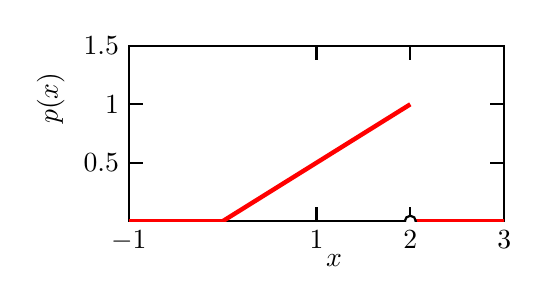
\begin{tikzpicture}
\begin{axis}[
x label style={anchor=west},
xlabel={$x$},
xtick       = {-1,1,2,3},
xticklabels = {$-1$,$1$,$2$,$3$},
xticklabel style={anchor=north},
y label style={anchor=south west},
ylabel={$p(x)$},
ytick       = {.5,1,1.5},
yticklabels = {$0.5$,$1$,$1.5$},
samples     = 320,
xmin =-1, xmax = 3,
ymin = 0, ymax = 1.5,
axis line style = {  thick, -},
every major tick/.append style={ thick, black, major tick length=5pt},
width=2.5in, height=1.5in
]
\addplot[domain=0:2, red, ultra thick, mark=none]{1/2*x};
\addplot[domain=-1:0, red, ultra thick, mark=none]{0};
\addplot[domain=2:3, red, ultra thick, mark=none]{0};
\filldraw[fill=white, thick] (2,0) circle (2pt);
\end{axis}
\end{tikzpicture}




\task Using the value of $c$ you found in b), find\\ $P(X\leq 3/2)$, i.e. the probability that $X$ takes on a value less than or equal to $1.5$.
\sol{
$\ds P(X\leq1.5)=\int_0^{3/2}\frac{x}{2}\;dx$
\al{
\int_0^{1.5}\frac{x}{2}\;dx&=\frac{x^2}{4}\Big|_0^{3/2}\\
&=\frac{(3/2)^2}{4}-\frac{0^2}{4}\\
&=\frac{9/4}{4}-0\\
&=\frac{9}{16}\\
&=0.5626\\
&=56.25\%
}
}


\task Give an example of an interval $[0,b]$ that $X$ has a $25\%$ chance of falling in. Show your answer is correct.
\sol{
We want $\ds \int_a^b\frac{x}{2}\;dx=\int_0^b \frac{x}{2}\;dx=0.25$.
\al{
\int_0^b \frac{x}{2}\;dx&=\frac{1}{4}\\
\frac{x^2}{4}\Big|0^b&=\frac{1}{4}\\
\frac{b^2}{4}-\frac{0^2}{4}&=\frac{1}{4}\\
\frac{b^2}{4}&=\frac{1}{4}\\
4\cdot\frac{b^2}{4}&=4\cdot \frac{1}{4}\\
b^2&=1\\
b&=\pm 1\\
}
We choose $b=1$ since $b=-1$ is not in the support.
}



}

%%%%%%%%%
\newpage%
%%%%%%%%%

{\bf\color{blue}Mini-lecture.} The {\bf cumulative distribution function} (CDF) of a continuous random variable $X$ measures how much probability has accumulated up to a given point.    Informally, it is the ``probability-so-far" function
\[F(x) = \unlineb{2}{\ds P(X\leq x)=\int_a^x p(w)\;dw}\]
\blue{Since we're defining a new function using an integral where the upper bound is the variable $x$, we cannot use $x$ in the integrand $p(x)$ because we would be using $x$ to represent two different quantities. Pick any other variable. We used $w$ here. That means $dx$ also becomes $dw$.}

\example{\bf\color{Orange}P2} Let's continue with the previous \blue{\bf Exercise B} with utilizing the probability density function and graph below.\\
\mpageT{.5}{.5}{\centering
$$
p(x) = 
\begin{cases} 
cx & \text{for } 0 \leq x \leq 2, \\
0 & \text{otherwise}.
\end{cases}
$$
\blue{From previous exercise, $c=\dfrac{1}{2}$}
}{\centering
\begin{tikzpicture}
\begin{axis}[
	x label style={anchor=west},
xlabel={$x$},
xtick       = {-1,1,1.5,2,3},
xticklabels = {$-1$,$1$,$ 1.5$,$2$,$3$},
xticklabel style={anchor=north},
y label style={anchor=south west},
ylabel={$p(x)$},
ytick       = {.5,1,1.5},
yticklabels = {$0.5$,$1$,$1.5$},
samples     = 320,
xmin =-1, xmax = 3,
ymin = -.1, ymax = 1.5,
axis line style = {  thick, ->},
every major tick/.append style={ thick, black, major tick length=5pt},
width=2.083in, height=1.25in
]
	\addplot[domain=0:2, red, ultra thick, mark=none]{x/2};
                \addplot[domain=2:3, red, ultra thick, ->]{0};
                \addplot[domain=-1:0, red, ultra thick, <-]{0};
                \filldraw[fill=white, thick] (2,0) circle (2.5pt);
                \filldraw[fill=red, thick] (2,1) circle (1.5pt);
	\addplot[name path=f, domain=0:1.5, red, ultra thick, mark=none]{x/2};
	   \path[name path=axis] (0,0) -- (1.5,0);
	    \addplot [
                thick,
                color=red!40,
                fill=red!40, 
                fill opacity =0.35
                ]
                fill between[
                of=f and axis,
                soft clip={domain=0:2},
                ];
\end{axis}
\end{tikzpicture}
}
\tasksA{2}{
\task Based on the definition we just learned, what is the cumulative distribution function $F(x)$ of the random variable $X$? You will want to use the value of $c$ found in the previous exercise.
\sol{
\al{
F(x)&=\int_0^x \frac{w}{2}\;dw\\
&=\frac{w^2}{4}\Bigg|_0^x\\
&=\frac{x^2}{4}-\frac{0^2}{4}\\
F(x)&=\frac{x^2}{4}
}
}
\task Find $F(3/2)$ and $F(2)$. These should be consistent with work done on the previous exercise.
\sol{
\al{
F(3/2)&=\frac{(3/2)^2}{4}=\frac{9/4}{4}=\frac{9}{16}
\intertext{We are seeing that $F(x)$ provides an easy way to calculate probabilities of the form $P(X\leq x)$. $F(3/2)$ is also the area in the graph above.}
F(2)&=\frac{2^2}{4}=1
\intertext{We know that the probability over the support must be $1$. So $F(2)=\int_0^2p(w)\;dw=1$ is consistent with Property $\#2$ of a continuous random variable. }
}
}
\task* Sketch the graph of $F(x)$. \blue{The graph of $F(x)=x^2/4$ is shown below right. Note that for $x<0$ $F(x)=0$ since we've accumulated no probability. For $x>2$, $F(x)=1$ since we've accumulated all probabilities when $x=2$.\\\\We can interpret $F(x)$ graphically in two ways. 1) $F(x)$ represents the area between $p(x)$ and the $x$-axis on $[a,x]=[0,x]$.  2) $F(x)$ represents the $y$-value on the graph of $F$ shown below right. }

\mpageT{.5}{.5}{\centering
\begin{tikzpicture}
\begin{axis}[
	x label style={anchor=west},
xlabel={$x$},
xtick       = {-1,1,1.25, 2,3},
xticklabels = {$-1$,$1$,$x$,$2$,$3$},
xticklabel style={anchor=north},
y label style={anchor=south west},
ylabel={$p(x)$},
ytick       = {.5,1,1.5},
yticklabels = {$0.5$,$1$,$1.5$},
samples     = 320,
xmin =-1, xmax = 3,
ymin = -.1, ymax = 1.5,
axis line style = {  thick, ->},
every major tick/.append style={ thick, black, major tick length=5pt},
width=2.5in, height=1.5in
]
	\addplot[domain=0:2, red, ultra thick, mark=none]{x/2};
		\addplot[name path=f, domain=0:1.25, red, ultra thick, mark=none]{x/2};
	   \path[name path=axis] (0,0) -- (1.25,0);
	    \addplot [
                thick,
                color=red!40,
                fill=red!40, 
                fill opacity =0.35
                ]
                fill between[
                of=f and axis,
                soft clip={domain=0:1.25},
                ];
                \addplot[domain=2:3, red, ultra thick, ->]{0};
                \addplot[domain=-1:0, red, ultra thick, <-]{0};
                \filldraw[fill=white, thick] (2,0) circle (2.5pt);
                \filldraw[fill=red, thick] (2,1) circle (1.5pt);
\end{axis}
\end{tikzpicture}
}{\centering
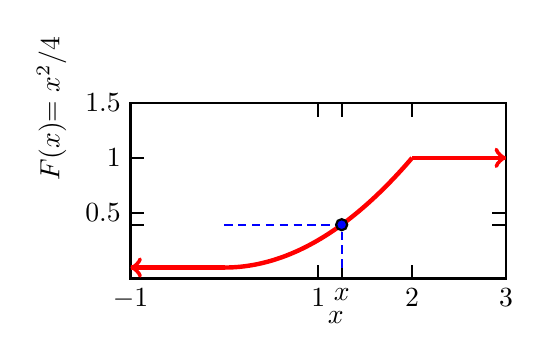
\begin{tikzpicture}
\begin{axis}[
	x label style={anchor=west},
xlabel={$x$},
xtick       = {-1, 1,1.25, 2,3},
xticklabels = {$-1$, $1$,$x$,$2$,$3$},
xticklabel style={anchor=north},
y label style={anchor=south west},
ylabel={$F(x)\blue{=x^2/4}$},
ytick       = {.390625,.5,1,1.5},
yticklabels = {, $0.5$,$1$ ,$1.5$},
samples     = 320,
xmin =-1, xmax = 3,
ymin = -.1, ymax = 1.5,
axis line style = {  thick, ->},
every major tick/.append style={ thick, black, major tick length=5pt},
width=2.5in, height=1.5in
]
\addplot[domain=0:2, red, ultra thick, mark=none]{x^2/4};
\addplot[domain=2:3, red, ultra thick, ->]{1};
    \addplot[domain=-1:0, red, ultra thick, <-]{0};
    \draw[densely dashed, blue, thick ] (1.25,0) -- (1.25,.390625);
    \draw[densely dashed, blue, thick ] (0,.390625) -- (1.25,.390625);
    \filldraw[fill=blue, thick] (1.25, .390625) circle (2pt);
\end{axis}
\end{tikzpicture}
}
\task* Find $P(1/2\leq X\leq 3/2)$ two ways:
}
\tasksI{2}{
\task Consider how the graph of $p(x)$ relates to this probability. 
\sol{
We can find this probability by finding the net area between $p(x)$ and the $x$-axis over $1/2 \leq x\leq 3/2$.
\al{
\int_{1/2}^{3/2} \frac{x}{2}\;dx&=\frac{x^2}{4}\Bigg|_{1/2}^{3/2}\\
&=\frac{3/2)^2}{4}-\frac{(1/2)^2}{4}\\&=\frac{9/4}{4}-\frac{1/4}{4}\\
&=\frac{9}{16}-\frac{1}{16}\\
&=\frac{8}{16}\\
&=\frac{1}{2}
}
This probability is represented by the area below.
\begin{tikzpicture}
\begin{axis}[
	x label style={anchor=west},
xlabel={$x$},
xtick       = {-1,.5,1,1.5, 2,3},
xticklabels = {$-1$,$.5$,$1$,$1.5$,$2$,$3$},
xticklabel style={anchor=north},
y label style={anchor=south west},
ylabel={$p(x)$},
ytick       = {.5,1,1.5},
yticklabels = {$0.5$,$1$,$1.5$},
samples     = 320,
xmin =-1, xmax = 3,
ymin = -.1, ymax = 1.5,
axis line style = {  thick, ->},
every major tick/.append style={ thick, black, major tick length=5pt},
width=2.5in, height=1.5in
]
	\addplot[domain=0:2, red, ultra thick, mark=none]{x/2};
		\addplot[name path=f, domain=.5:1.5, red, ultra thick, mark=none]{x/2};
	   \path[name path=axis] (.5,0) -- (1.5,0);
	    \addplot [
                thick,
                color=red!40,
                fill=red!40, 
                fill opacity =0.35
                ]
                fill between[
                of=f and axis,
                soft clip={domain=.5:1.5},
                ];
\addplot[domain=2:3, red, ultra thick, ->]{0};
	\addplot[domain=-1:0, red, ultra thick, <-]{0};
	          \filldraw[fill=white, thick] (2,0) circle (2.5pt);
	                    \filldraw[fill=red, thick] (2,1) circle (1.5pt);
\end{axis}
\end{tikzpicture}
}
\task Consider how $F(x)$ can be used to find this probability.
\sol{
\al{
P(1/2\leq X\leq 3/2)&=F(3/2)-F(1/2)\\
&=\frac{9}{16} -\frac{(1/2)^2}{4}  
\intertext{(from prior work,  $F(3/2)=\dfrac{9}{16}$)}
&=\frac{9}{16}-\frac{1/4}{4}\\
&=\frac{9}{16}-\frac{1}{16}\\
&=\frac{8}{16}\\&=\frac{1}{2}
}
Thus $P(1/2\leq X\leq 3/2)=50\%$
}
}


\newpage
\exercise{\bf\color{Orange}P2}
The probability density function of a random variable $X$ is given below:
\[
p(x) = 
\begin{cases} 
3x^2 & \text{for } 0 \leq x \leq 1, \\
0 & \text{otherwise},
\end{cases}
\]
\tasksA{2}{
\task* Find and graph the cumulative distribution function $F(x)$.\\
\mpageT{.6}{.4}{
\sol{
Support is $0\leq x\leq 1$
\al{
F(x)&=\int_0^x 3w^2\;dw\\
&=w^3\Big|_0^x\\
&=x^3-0^3\\
F(x)&=x^3
}
}
}{
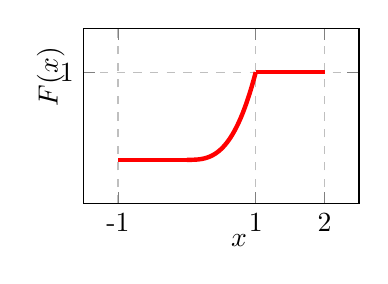
\begin{tikzpicture}
\begin{axis}[
xlabel = {$x$},
x label style={anchor=west},
ylabel = {$F(x)$},
y label style={anchor=west},
xtick       = {-1,1,2},
xticklabels = {-1,1,2},
ytick       = {1,2},
yticklabels = {1,2},
samples     = 160,
domain      = -1:3,
restrict y to domain=-0.1:4,
xmin = -1.5, xmax = 2.5,
ymin = -0.5, ymax = 1.5,
width = 2in, height=1.5in,
grid=both, grid style=dashed
]
                    \addplot[domain=0:1, red, ultra thick, mark=none]{x^3};
 \addplot[domain=-1:0, red, ultra thick, mark=none]{0};
  \addplot[domain=1:2, red, ultra thick, mark=none]{1};
\end{axis}
\end{tikzpicture}
~\\
\blue{
Note that 
\itemI{
\item For $x<0$, $F(x)=0$
\item For $x>1$, $F(x)=1$
}
}
}
\task Utilize $F(x)$ to find $P(X\leq 1/4)$
\sol{
\al{ 
P(X\leq 1/4)&=\int_0^{1/4}3x^2\;dx\\
&=F(1/4)\\
&=(1/4)^3\\
&=\frac{1}{64} 
}
}
\task What is $P(X>1/4)$? Consider how property $\#2$ of a continuous random variable might be helpful.
\sol{\\
We know that  $P(X\leq 1/4)+P(X> 1/4) =1$. So 
\al{
P(X> 1/4) &=1-P(X\leq 1/4)\\
&=1-\frac{1}{64}\\
&=\frac{63}{64}
}
}
\task What is $P(1/4\leq X \leq 1/2)$?
\sol{
\al{
P(1/4\leq X \leq 1/2)&=P(X \leq 1/2)-P(X\leq 1/4)\\
&=F(1/2)-F(1/4)\\
&=(1/2)^3-(1/4)^3\\
&=\frac{1}{8}-\frac{1}{64}\\
&=\frac{8}{64}-\frac{1}{64}\\
&=\frac{7}{64}
}
Alternatively, we can consider 
\al{
P(1/4\leq X \leq 1/2)&=\int_{1/4}^{1/2} 3x^2\;dx\\
\intertext{$F(x)$ is an anti-derivative of $3x^2$ so we can use the FTOC}
&=F(1/2)-F(1/4)\\
%&=(1/2)^3-(1/4)^3\\
&=\frac{7}{64}
}
}
\task Find $b$ so that $P(X\leq b)=\dfrac{8}{27}$
\sol{
We want 
\al{
\int_0^b 3x^2\;dx&=\frac{8}{27}\\
F(b)&=\frac{8}{27}\\
b^3&=\frac{8}{27}\\
b&=\left(\frac{8}{27}\right)^{1/3}\\
b&=\frac{8^{1/3}}{(27)^{1/3}}\\
&=\frac{2}{3}
}
Thus $\ds P(X\leq 2/3)=\frac{8}{27}$
}
}


%%%%%%%%%
\newpage%
%%%%%%%%%

\exercise{\bf\color{Orange}P2}
%%%%%EXERCISE D%%%%%%%%%%%%%%%%
The probability density function of a random variable $Z$ and its graph are given below:
\mpageT{.5}{.5}{
\[
p(z) = 
\begin{cases} 
\dfrac{3}{14}  \sqrt{z}& \text{for } 1 \leq z \leq 4, \\
0 & \text{otherwise}
\end{cases}
\]
}{\centering
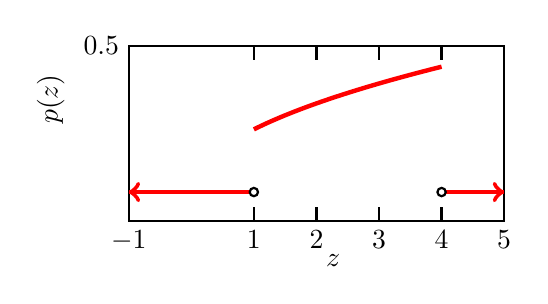
\begin{tikzpicture}
\begin{axis}[
	x label style={anchor=west},
xlabel={$z$},
xtick       = {-1,1,2,3,4,5},
xticklabels = {$-1$,$1$,$2$,$3$,$4$,$5$},
xticklabel style={anchor=north},
y label style={anchor=south west},
ylabel={$p(z)$},
ytick       = {.5, 9/16,1,1.5},
yticklabels = {$0.5$,,$1$,$1.5$},
samples     = 320,
xmin =-1, xmax = 5,
ymin = -.1, ymax = .5,
axis line style = {  thick, ->},
every major tick/.append style={ thick, black, major tick length=5pt},
width=2.5in, height=1.5in
]
\addplot[domain=1:4, red, ultra thick, mark=none]{ 3/14*sqrt(x) };
\addplot[domain=4:5, red, ultra thick, ->]{0};
    \addplot[domain=-1:1, red, ultra thick, <-]{0};
     \filldraw[fill=white, thick] (1,0) circle (1.5pt);
                      \filldraw[fill=white, thick] (4,0) circle (1.5pt);
\end{axis}
\end{tikzpicture}
}

\tasksA{2}{
\task Find the cumulative distribution function $F(z)$
\sol{
\al{
F(z)&=\int_1^{z} \frac{3}{14}  \sqrt{w}\;dw
\intertext{We cannot use the variable $z$ in both the upper bound and in the integrand/interior of the integral. We must choose any other variable. Here the variable $w$ was used to represent the integrand as $\dfrac{3}{14}  \sqrt{w}$. }
F(z)&=\frac{3}{14}\int_1^{z}   w^{1/2}\;dw\\
&=\frac{3}{14}\cdot \frac{w^{3/2}}{3/2}\Bigg|_1^z\\
&=\frac{3}{14}\cdot \frac{2}{3}w^{3/2}\Bigg|_1^z\\
&=\frac{1}{7}w^{3/2}\Bigg|_1^z\\
&=\frac{1}{7}z^{3/2}-\frac{1}{7}1^{3/2}\\
&=\frac{1}{7}z^{3/2}-\frac{1}{7}
}
}
\task Find $P( Z \leq 9/4)$
\sol{
\al{
P( Z \leq 9/4)&=F(9/4)\\
&=\frac{1}{7}(9/4)^{3/2} -\frac{1}{7}\\
&=\frac{1}{7}(\sqrt{9/4})^{3} -\frac{1}{7}\\
&=\frac{1}{7}(3/2)^{3} -\frac{1}{7}\\
&=\frac{1}{7}\cdot \frac{27}{8} -\frac{1}{7}\\
&=\frac{1}{7}\left(  \frac{27}{8} -1 \right)\\
&=\frac{1}{7}\left(  \frac{27}{8} -\frac{8}{8} \right)\\
&=\frac{1}{7}\left(  \frac{19}{8}  \right)\\
&=\frac{19}{56}\\
&\approx 0.3393\\
&=33.93\%
}
}
}
\vs{3}

{\bf\color{blue}Extra Practice 1.} \ltrm{\bf\color{Orange}P2}
The PDF of the continuous random variable $X$ is given below:\\

\

\,\hfill
%
\begin{minipage}[t][0.5in]{0.25\textwidth}
$
p(x) = 
\begin{cases} 
1 & \text{for } 0 \leq x \leq 1, \\
0 & \text{otherwise},
\end{cases}
$
\end{minipage}
%
\hfill
%
\begin{minipage}[t][0.5in]{0.25\textwidth}
\,\\[-0.5in]
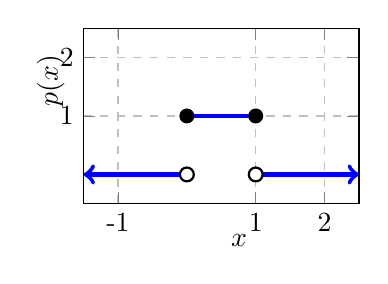
\begin{tikzpicture}
\begin{axis}[
%    axis y line = left,
%    axis x line = bottom,
xlabel = {$x$},
x label style={anchor=west},
ylabel = {$p(x)$},
y label style={anchor=west},
xtick       = {-1,1,2},
xticklabels = {-1,1,2},
ytick       = {1,2},
yticklabels = {1,2},
samples     = 160,
domain      = -1:3,
xmin = -1.5, xmax = 2.5,
ymin = -0.5, ymax = 2.5,
width = 2in, height=1.5in,
grid=both, grid style=dashed
]
\draw[ultra thick,blue,<-] (-1.5,0) -- (0,0);
\draw[ultra thick,blue] (0,1) -- (1,1);
\draw[ultra thick,blue,->] (1,0) -- (2.5,0);
\filldraw (0,1) circle (2.5pt);
\filldraw (1,1) circle (2.5pt);
\filldraw[fill=white, thick] (1,0) circle (2.5pt);
\filldraw[fill=white, thick] (0,0) circle (2.5pt);
\end{axis}
\end{tikzpicture}
\end{minipage}
%
\hfill\,\\

\begin{itemize}
\item[(a)] Find the CDF $F(x)$ of $X$.

\sol{
\al{
F(x)=\int_0^x p(w)\;dw&=\int_0^x 1\;dw\\
&=w\Big|_0^x\\
&=x=0\\
F(x)=x
}
}


\end{itemize}

\begin{minipage}[t]{0.5\textwidth}
\begin{itemize}
\item[(b)] Sketch the graph of the CDF $F(x)$.

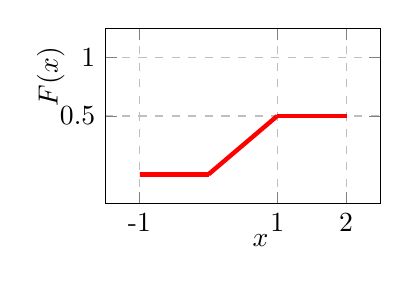
\begin{tikzpicture}
\begin{axis}[
xlabel = {$x$},
x label style={anchor=west},
ylabel = {$F(x)$},
y label style={anchor=west},
xtick       = {-1,1,2},
xticklabels = {-1,1,2},
ytick       = {1,2},
yticklabels = {0.5,1},
samples     = 160,
domain      = -1:3,
xmin = -1.5, xmax = 2.5,
ymin = -0.5, ymax = 2.5,
width = 2in, height=1.5in,
grid=both, grid style=dashed
]
\addplot[domain=0:1, red, ultra thick, mark=none]{x};
\addplot[domain=-1:0, red, ultra thick, mark=none]{0};
\addplot[domain=1:2, red, ultra thick, mark=none]{1};
\end{axis}
\end{tikzpicture}
\end{itemize}
\blue{Note that for $x<0$, $F(x)=0$.  \\When $x>1$, $F(x)=1$}
\end{minipage}
%
\begin{minipage}[t]{0.45\textwidth}
\begin{itemize}
\item[(c)] Find the number $m$ for which $P(X<m)=0.5$. ({\bf Note:} this number $m$ is called the {\bf median} of $X$.)
\sol{
We want $$\ds \int_0^m 1\;dx=0.5$$ We can alternatively write this as 
\al{
F(m)&=0.5\\
m&=0.5
}
Thus $(P(X\leq 0.5)=0.5$
}
\end{itemize}
\end{minipage}

\newpage

{\bf\color{blue}Extra Practice 2.} \ltrm{\bf\color{Orange}P2}Consider the following probability density function for a random variable $X$:
\[
p(x) = 
\begin{cases} 
cx(1 - x) & \text{for } 0 \leq x \leq 1, \\
0 & \text{otherwise}.
\end{cases}
\]
\tasksA{2}{
\task Find the value of $c$ making $f$ a valid probability density function.

\sol{
The support is $S=[0,1]$. We use Property $\#2$ of a continuous random variable.
\al{
\int_0^1 cx(1-x)\;dx&=1\\
c\int_0^1 x-x^2\;dx&=1\\
c\left[\frac{x^2}{2}-\frac{x^3}{3}\Bigg|_0^1\right]&=1\\
c\left[\left( \frac{1^2}{2}-\frac{1^3}{3}\right)- \left( \frac{0^2}{2}-\frac{0^3}{3}\right)  \right]&=1\\
c\left[\left( \frac{1}{2}-\frac{1}{3}\right)- 0  \right]&=1\\
c\left[ \frac{3}{6}-\frac{2}{6}  \right]&=1\\
    c\left[ \frac{1}{6} \right]&=1\\
    c&=6
}
Thus 
\[
p(x) = 
\begin{cases} 
6x(1 - x) & \text{for } 0 \leq x \leq 1, \\
0 & \text{otherwise}.
\end{cases}
\]
}

\task Suppose you know $X$ has a 75\% chance to fall in the interval $[a,1]$. Find $a$.

\sol{
We want 
\al{
\int_a^16x(1 - x) \;dx &=\frac{3}{4}\\
6\int_a^1 x-x^2 \;dx &=\frac{3}{4}\\
6\left[ \frac{x^2}{2}-\frac{x^3}{3}\Bigg|_a^1\right]&=\frac{3}{4}\\
6\left[ \left( \frac{1^2}{2}-\frac{1^3}{3} \right)   -   \left( \frac{a^2}{2}-\frac{a^3}{3} \right) \right]&=\frac{3}{4}\\
6\left[ \left( \frac{1}{2}-\frac{1}{3} \right)   -   \left( \frac{a^2}{2}-\frac{a^3}{3} \right) \right]&=\frac{3}{4}\\
6\left[ \left( \frac{3}{6}-\frac{2}{6} \right)   -   \left( \frac{3a^2}{6}-\frac{2a^3}{6} \right) \right]&=\frac{3}{4}\\
6\left[  \frac{1}{6}   -   \frac{3a^2-2a^3}{6} \right]&=\frac{3}{4}
\intertext{Distribute $6$ through left side.}
\left[   1 -   (3a^2-2a^3) \right]&=\frac{3}{4}\\
1 -   3a^2+2a^3 &=\frac{3}{4}\\
2a^3-3a^2+1-\frac{3}{4} &=0\\
2a^3-3a^2+\frac{1}{4} &=0\\
}
Solving a cubic equation by hand is not an expectation of this course. Using technology (Desmos will work well) allows us to find three roots to this equation. Only one is in the support $0\leq x\leq 1$: $x=a\approx 0.3564$ This means that $$\int_{0.3264}^1 6x(1-x)\;dx \approx 0.75$$
}

%%%%%%%%%
%\newpage%
%%%%%%%%%

\task* Suppose you know $X$ has a 25\% chance to fall in the interval $[0,b]$. Find $b$.
\sol{ Property $\#2$ of continuous random variables ensures that 
\al{
\int_{0}^1 6x(1-x)\; dx&=1
\intertext{The break-apart property of definite integrals means}
\int_0^{0.3264} 6x(1-x)\; dx+\int_{0.3264}^1 6x(1-x)\; dx&=1
\intertext{Since $\ds \int_{0.3264}^1 6x(1-x)\; dx=0.75$, it must be the case that }
\int_0^{0.3264} 6x(1-x)\; dx&=0.25
}
Thus $b=0.3264$
}


}

\newpage
{\bf\color{blue}Extra Practice 3.} \ltrm{\bf\color{Orange}P2}
Suppose we want to analyze the fishing industry in a small town. Each day, the boats bring back at least 2 tons of fish, but never more than 8 tons.

Suppose $X$ is the continuous random variable for the amount of fish brought back by the boats on a day. The following figure shows the the probability density function $p(x)$ of $X$. 

\begin{center}
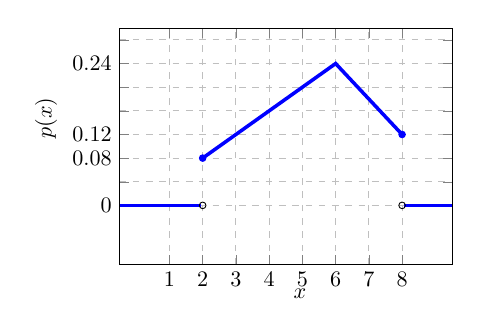
\begin{tikzpicture}[scale=.8]
\begin{axis}[
x label style={anchor=west},
xlabel={$x$},
xticklabel style={anchor=north},
y label style={anchor=south west},
ylabel={$p(x)$},
xtick       = {1,2,3,4,5,6,7,8},
xticklabels = {$1$,$2$,$3$,$4$,$5$,$6$,$7$,$8$},
ytick       = {0, 0.04, 0.08, 0.12, 0.16, 0.2, 0.24, 0.28},
yticklabels = {$0$, , $0.08$, $0.12$, ,,$0.24$, ,},
samples     = 320,
domain      = -1:9.5,
restrict y to domain=-3.5:2.5,
xmin = -0.5, xmax = 9.5,
ymin = -0.1, ymax = 0.3,
height=2.1in, width=2.7in,
grid=both, grid style=dashed
]
\draw[ultra thick, blue,-] (2,0.08) -- (6,0.24) -- (8,0.12);
\draw[ultra thick, blue,-] (-0.5,0) -- (1.95,0);
\draw[ultra thick, blue,-] (8.05,0) -- (9.5,0);
\draw (2,0) circle (1.5pt);
\draw (8,0) circle (1.5pt);
\draw[blue,fill=blue] (2,0.08) circle (1.5pt);
\draw[blue,fill=blue] (8,0.12) circle (1.5pt);
\end{axis}
\end{tikzpicture}
\end{center}

\begin{enumerate}
\item[(a)] Find and graph the corresponding cumulative distribution function.

\sol{
We will first find a function for  $p(x)$. It will be a piecewise function and thus $F(x)$ will also be piecewise.\\
{\bf \em Finding $p(x)$}
\itemI{
\item For the interval $2\leq x\leq 6$, we will find the equation of a line in the form $p(x)=mx+b$ by using $2$ points: $(2,0.08)$ and $(6,0.24)$.
\al{
m=\frac{0.24-0.08}{6-2}=\frac{0/16}{4}=0.04
}
Thus $p(x)=0.04x+b$. \\Using the point $(6,(0.24)$, $$0.24=(0.04)\cdot 6+b\Rightarrow b=0.24-0.24=0.$$ On the interval $2\leq x\leq 6$, $$p(x)=0.04x$$
\item For the interval $6\leq x\leq 8$, we will find the equation of a line in the form $p(x)=mx+b$ by using $2$ points:  $(6,0.24)$ and $(8,0.12)$.
\al{m=\frac{0.12-0.24}{8-6}=\frac{-0.12}{2}=-0.06 }
Thus $$p(x)=-0.06x+b$$
We solve for $b$ by using $(6,0.24)$
$$0.24=-0.06\cdot 6+b\Rightarrow b=0.24+0.36=0.60$$
On  the interval $6\leq x\leq 8$, $$p(x)=-0.06x+0.6$$
}
We have found 
\[
p(x) = 
\begin{cases} 
0.04x & \text{for } 2 \leq x \leq 6, \\
-0.06+0.6 & \text{for } 6 < x\leq 8, \\
0 & \text{otherwise}.
\end{cases}
\]

{\bf \em Finding $F(x)$}\\
\itemI{
\item On the  interval $2\leq x\leq 6$ we use the first piece of $p(x)$
\al{
F_1(x)&=\int_2^x 0.04w\;dw\\
&=0.04\frac{w^2}{2}\Bigg|_2^x\\
&=0.02w^2\Bigg|_2^x\\
&=0.02x^2-0.02(2)^2\\
F_1&=0.02x^2-0.08
} 
\mpageT{.5}{.5}{
\item We point out that the area over  $2\leq x\leq 6$ is $$F_1(6)=0.02(6^2)-0.08=0.72-0.08=0.64.$$
\item On the  interval $6\leq x\leq 8$ we use the  second piece of $p(x)$.
\al{
F_2(x)=\int_6^x -0.06w+0.6\;dw&=-0.06\frac{w^2}{2}+0.6w\Bigg|_6^x\\
&=-0.03w^2+0.6w\Bigg|_6^x\\
&=\left(-0.03x^2+0.6x  \right)-\left(-0.03(6^2)+0.6(6)  \right)\\
&=\left(-0.03x^2+0.6x  \right)-\left(-1.08+3.6  \right)\\
&=\left(-0.03x^2+0.6x  \right)-\left(2.52  \right)\\
F_2(x)&=-0.03x^2+0.6x-2.52
}
Since $F(x)$ is the ``probability so far", we will need to add the area over the interval $2\leq x\leq 6$ to $F(2(x)$. That is
$$F_{2\;final}(x)=F_1(6)+F_2(x)=0.64-0.03x^2+0.6x-2.52=-0.03x^2+0.6x-1.88$$
}{\hs{-.5}
\begin{tikzpicture}[scale=1]
\begin{axis}[
x label style={anchor=west},
xlabel={$x$},
xticklabel style={anchor=north},
y label style={anchor=south west},
ylabel={$p(x)$},
xtick       = {1,2,3,4,5,6,7,8},
xticklabels = {$1$,$2$,$3$,$4$,$5$,$6$,$7$,$8$},
ytick       = {0, 0.04, 0.08, 0.12, 0.16, 0.2, 0.24, 0.28},
yticklabels = {$0$, , $0.08$, $0.12$, ,,$0.24$, ,},
samples     = 320,
domain      = -1:9.5,
restrict y to domain=-3.5:2.5,
xmin = -0.5, xmax = 9.5,
ymin = -0.1, ymax = 0.3,
height=2.1in, width=2.7in,
grid=both, grid style=dashed
]
  \addplot[ name path=f, domain=2:6,  blue, ultra thick, -, ] {.04*x  };
  \addplot[ name path=f, domain=6:8,  blue, ultra thick, -, ] {-.06*x+.6  };
\draw[ultra thick, blue,-] (8.05,0) -- (9.5,0);
\draw (2,0) circle (1.5pt);
\draw (8,0) circle (1.5pt);
\draw[blue,fill=blue] (2,0.08) circle (1.5pt);
\draw[blue,fill=blue] (8,0.12) circle (1.5pt);
  \addplot[ name path=f, domain=2:6,  blue, ultra thick, -, ] {.04*x  };
	   \path[name path=axis] (2,0) -- (6,0);
	    \addplot [
thick,
color=blue!20,
fill=blue!20, 
fill opacity=0.35
]
fill between[
of=f and axis,
soft clip={domain=2:6},
];
\node at (4.1,0.07)  {$F(6)=0.64$};
\end{axis}
\end{tikzpicture}
}
}

\mpageT{.5}{.5}{
We have found 
\[
F(x) = 
\begin{cases} 
0.02x^2-0.08 & \text{for } 2 \leq x \leq 6, \\
-0.03x^2+0.06x+2.2 & \text{for } 6 < \leq 8, \\
0 & \text{for } x<0\\
1 & \text{for } x>8
\end{cases}
\]
}{
The graph of $F(x)$ is \\
\begin{tikzpicture}[scale=1]
\begin{axis}[
x label style={anchor=west},
xlabel={$x$},
xticklabel style={anchor=north},
y label style={anchor=south west},
ylabel={$p(x)$},
xtick       = {1,2,3,4,5,6,7,8},
xticklabels = {$1$,$2$,$3$,$4$,$5$,$6$,$7$,$8$},
ytick       = {.16,.32,.48,.64,.80,.96,1.12},
yticklabels = { , $0.32$,  ,$0.64$, ,$0.96$, },
samples     = 320,
domain      = -1:9.5,
restrict y to domain=-3.5:2.5,
xmin = -0.5, xmax = 9.5,
ymin = -0.1, ymax = 1.12,
height=2.1in, width=2.7in,
grid=both, grid style=dashed
]
  \addplot[ name path=f, domain=-.5:2,  blue, ultra thick, <-, ] {0  };
    \addplot[ name path=f, domain=8:9.5,  blue, ultra thick, ->, ] {1  };
  \addplot[ name path=f, domain=2:6,  blue, ultra thick, -, ] {.02*x^2-0.08  };
    \addplot[ name path=f, domain=6:8,  blue, ultra thick, -, ] {-.03*x^2+0.6*x-1.88  };
    \draw[red,fill=red] (6,0.64) circle (2.pt);
\end{axis}
\end{tikzpicture}
}
}

\item[(b)] What is the probability that the catch of the day is between 5 and 7 tons?
\sol{
\al{
P(5\leq X\leq 7)=\int_5^6p(x)\;dx&=F(7)-F(5)\\
&=\left(  -0.03\cdot (7^2)+0.6(7)-1.88  \right) - \left( 0.02\cdot (5^2)-0.08 \right)
\intertext{(using technology to evaluate!)}
&=0.85-0.42\\
&=0.43
}
There is a $43\%$ chance the catch of the day is between $5$ and $7$ tons.
}

\vfill
\end{enumerate}



\end{document}

